\documentclass{article}
\usepackage{amsmath}  % 数学符号包
\usepackage{amssymb}  % 更多数学符号
\usepackage{enumitem} % 列表样式
\usepackage{fancyhdr} % 页眉设置
\usepackage{geometry} % 页面设置
\usepackage[UTF8]{ctex}
\usepackage{caption}
\usepackage{bm}
\usepackage{amsthm}
\usepackage{graphicx}
\everymath{\displaystyle}  % 让所有数学模式都使用 \displaystyle
\newcommand{\lb}{\left\llbracket}
\newcommand{\rb}{\right\rrbracket}


\geometry{a4paper, margin=1in}


\pagestyle{fancy}
\fancyhf{}
\fancyhead[C]{电子技术与系统 -- 实验累积报告}
\fancyhead[R]{2025.5}


\title{电子技术与系统 -- 实验累积报告}
\author{Noflowerzzk}
\date{2025.5}


\begin{document}
\maketitle

\section{电路基础}

\subsection{基尔霍夫电路定律}

\begin{figure}[htbp]
    \centering
    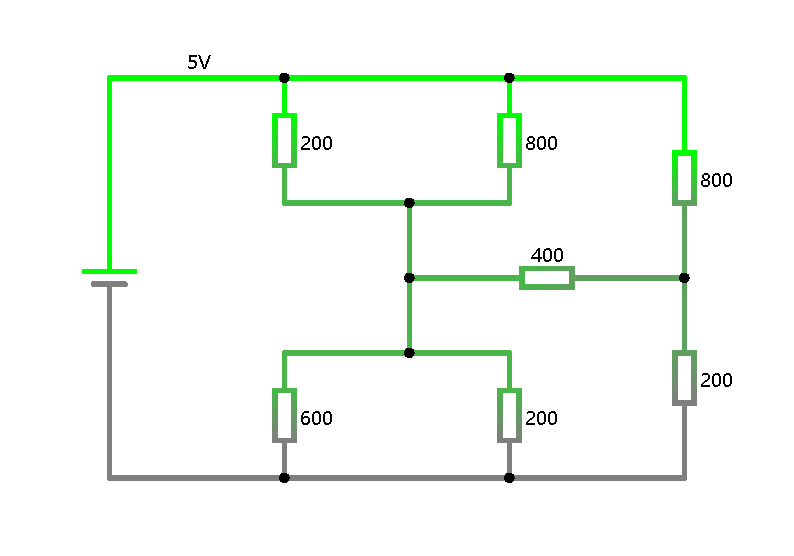
\includegraphics[width=0.5\textwidth]{KICL.pdf}
    \caption{KCL/KVL 验证}
\end{figure}

\section{晶体管输入输出特性}

\begin{figure}[htbp]
    \centering
    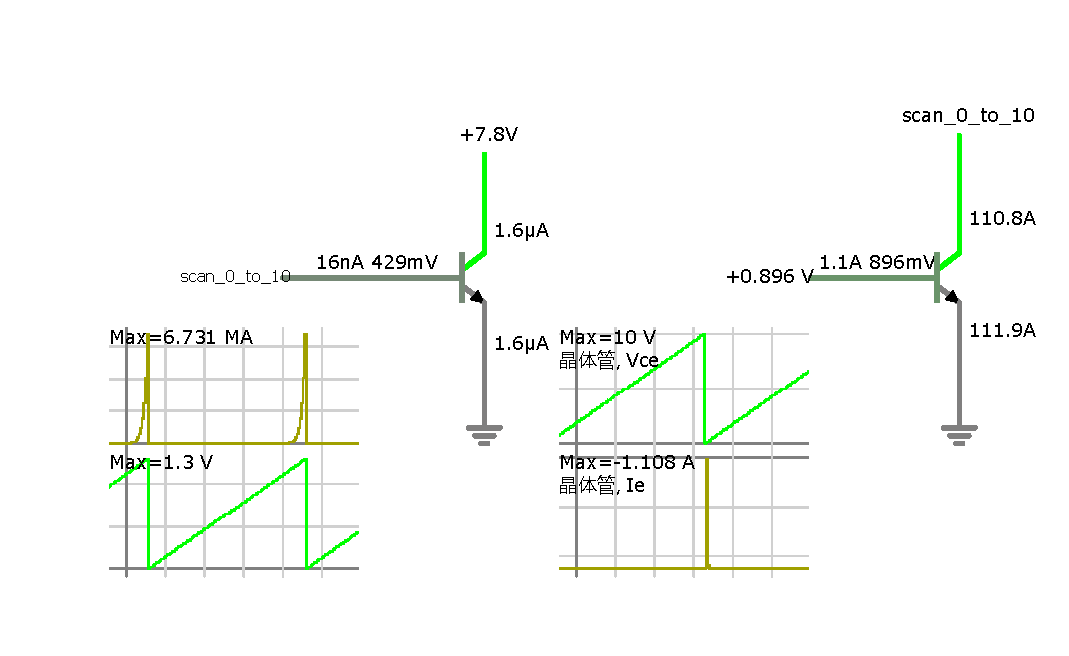
\includegraphics[width=0.7\textwidth]{晶体管输入输出.pdf}
    \caption{晶体管输入输出特性}
\end{figure}

最大电压 $0.149 \mathrm{V}$

\section{基本放大电路}

\begin{figure}[htbp]
    \centering
    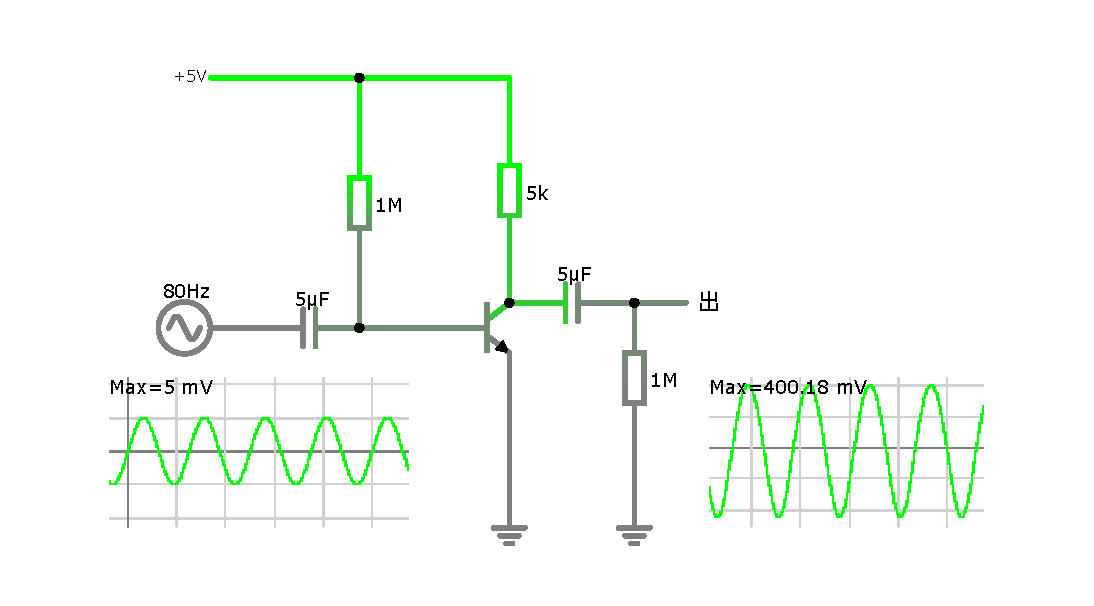
\includegraphics[width=0.7\textwidth]{基本放大电路.pdf}
    \caption{基本放大电路}
\end{figure}

更改输入为频率80Hz、幅值50mV的交流源时,波形出现明显失真,

\begin{figure}[htbp]
    \centering
    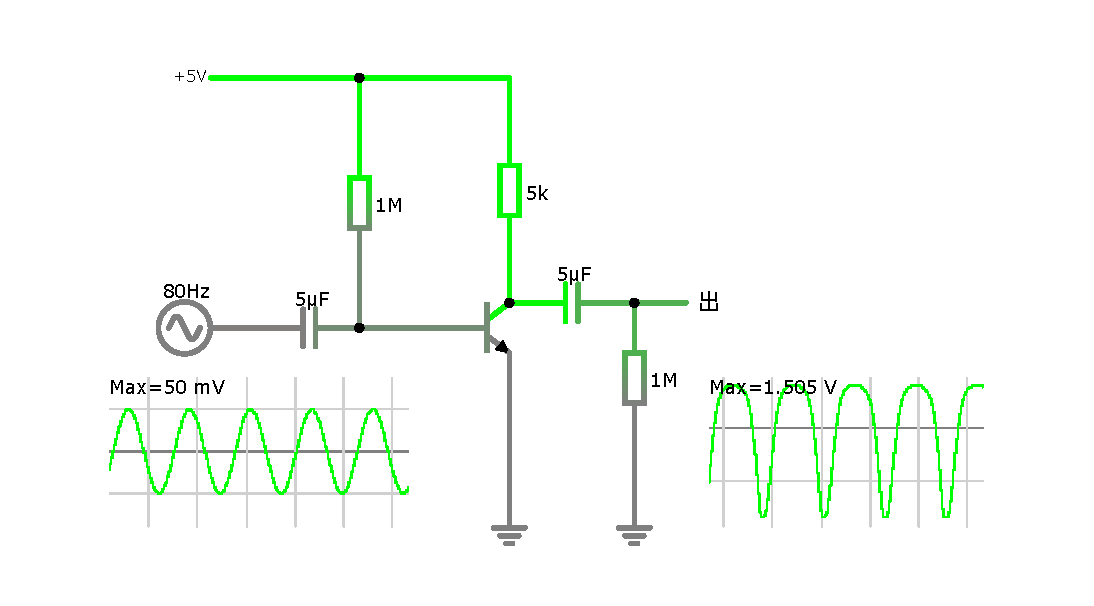
\includegraphics[width=0.7\textwidth]{基本放大电路_失真.pdf}
    \caption{基本放大电路 -- 失真}
\end{figure}

\section{CMOS 与非门电路}

\begin{figure}[htbp]
    \centering
    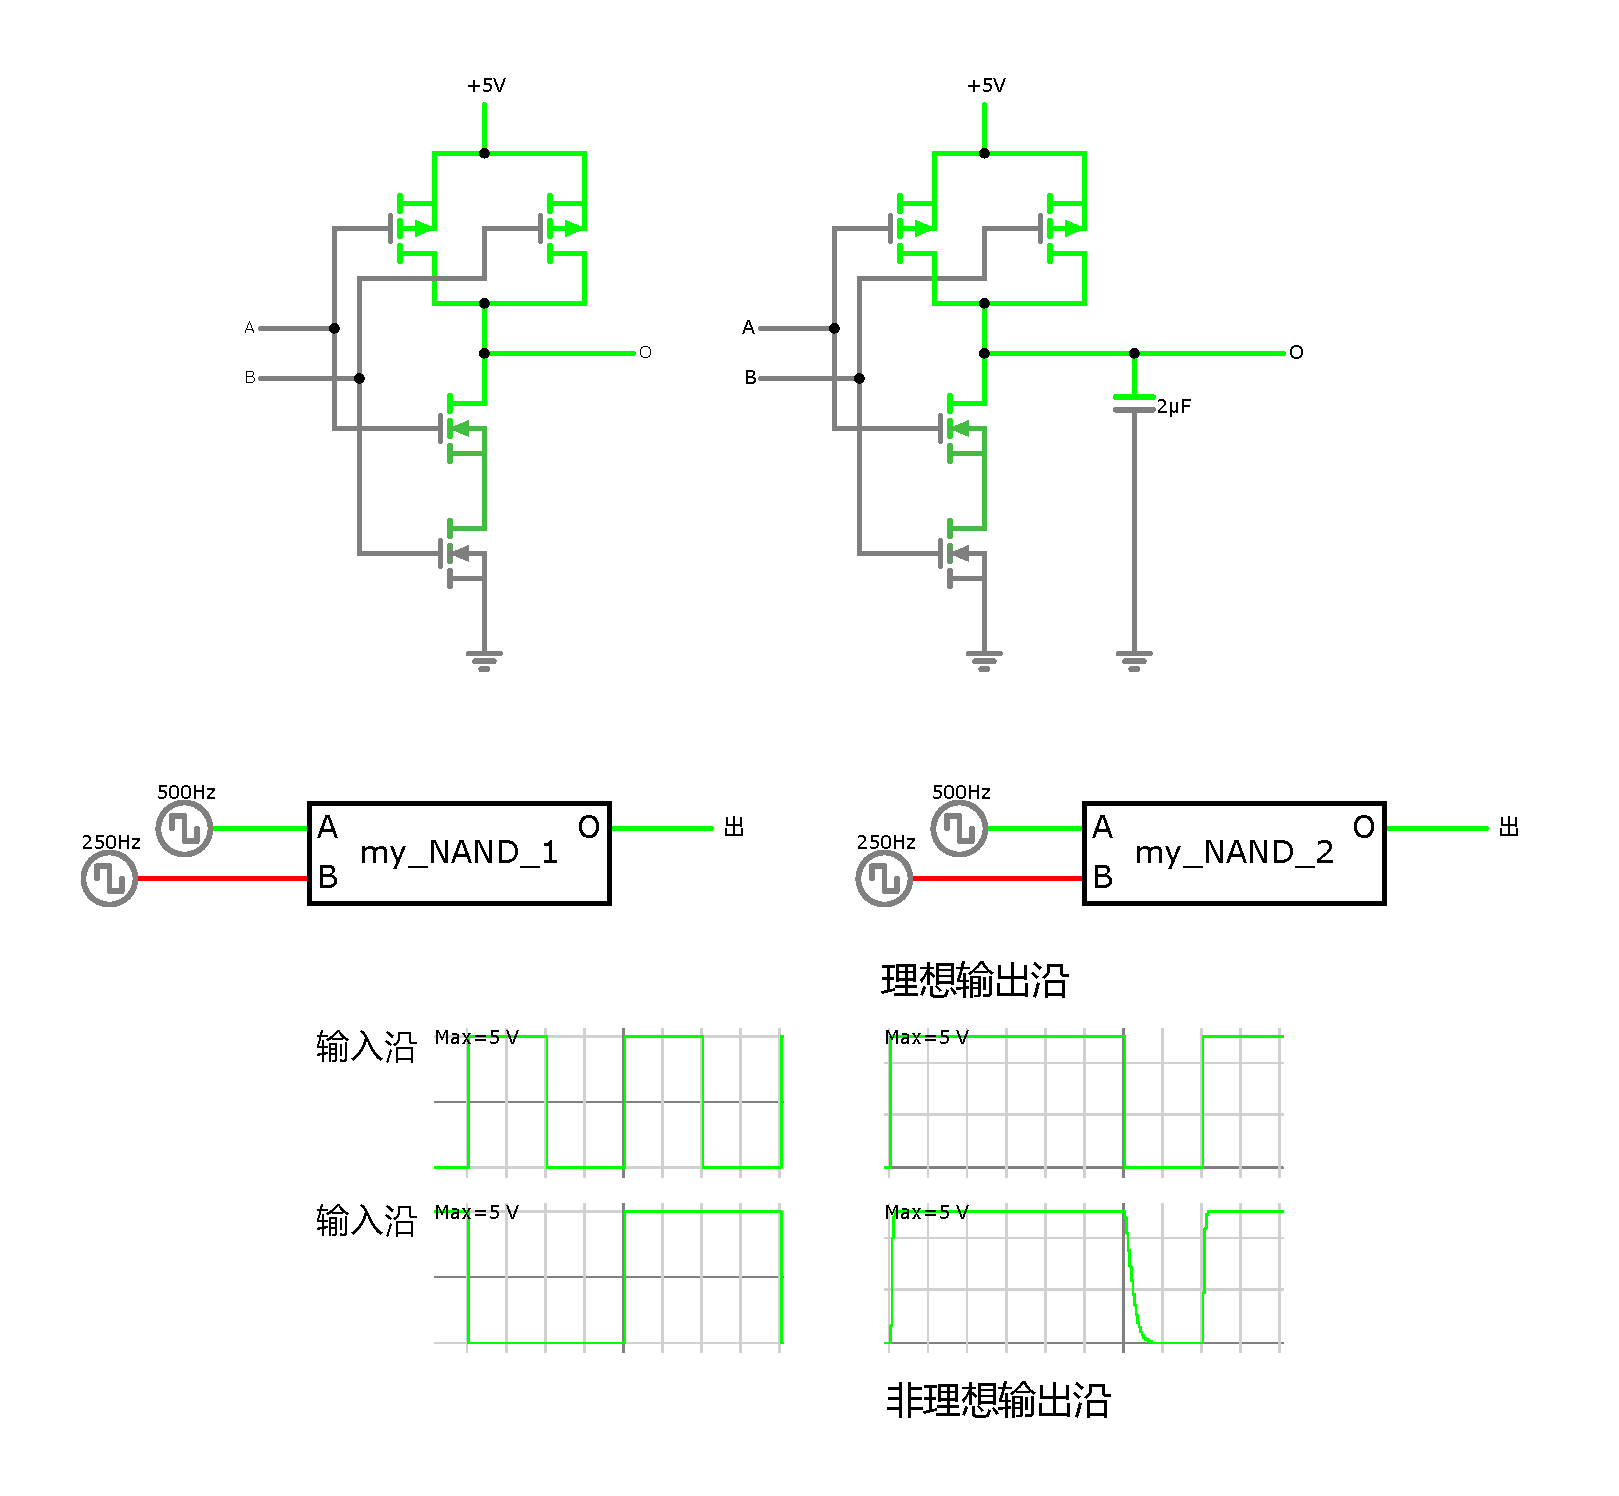
\includegraphics[width=0.7\textwidth]{NAND.pdf}
    \caption{CMOS 与非门电路}
\end{figure}

$t_{HL} = 0.45 \mathrm{ms}$, $t_{LH} = 0.10 \mathrm{ms}$

\section{半加器与全加器}

% \begin{figure}[htbp]
%     \centering
%     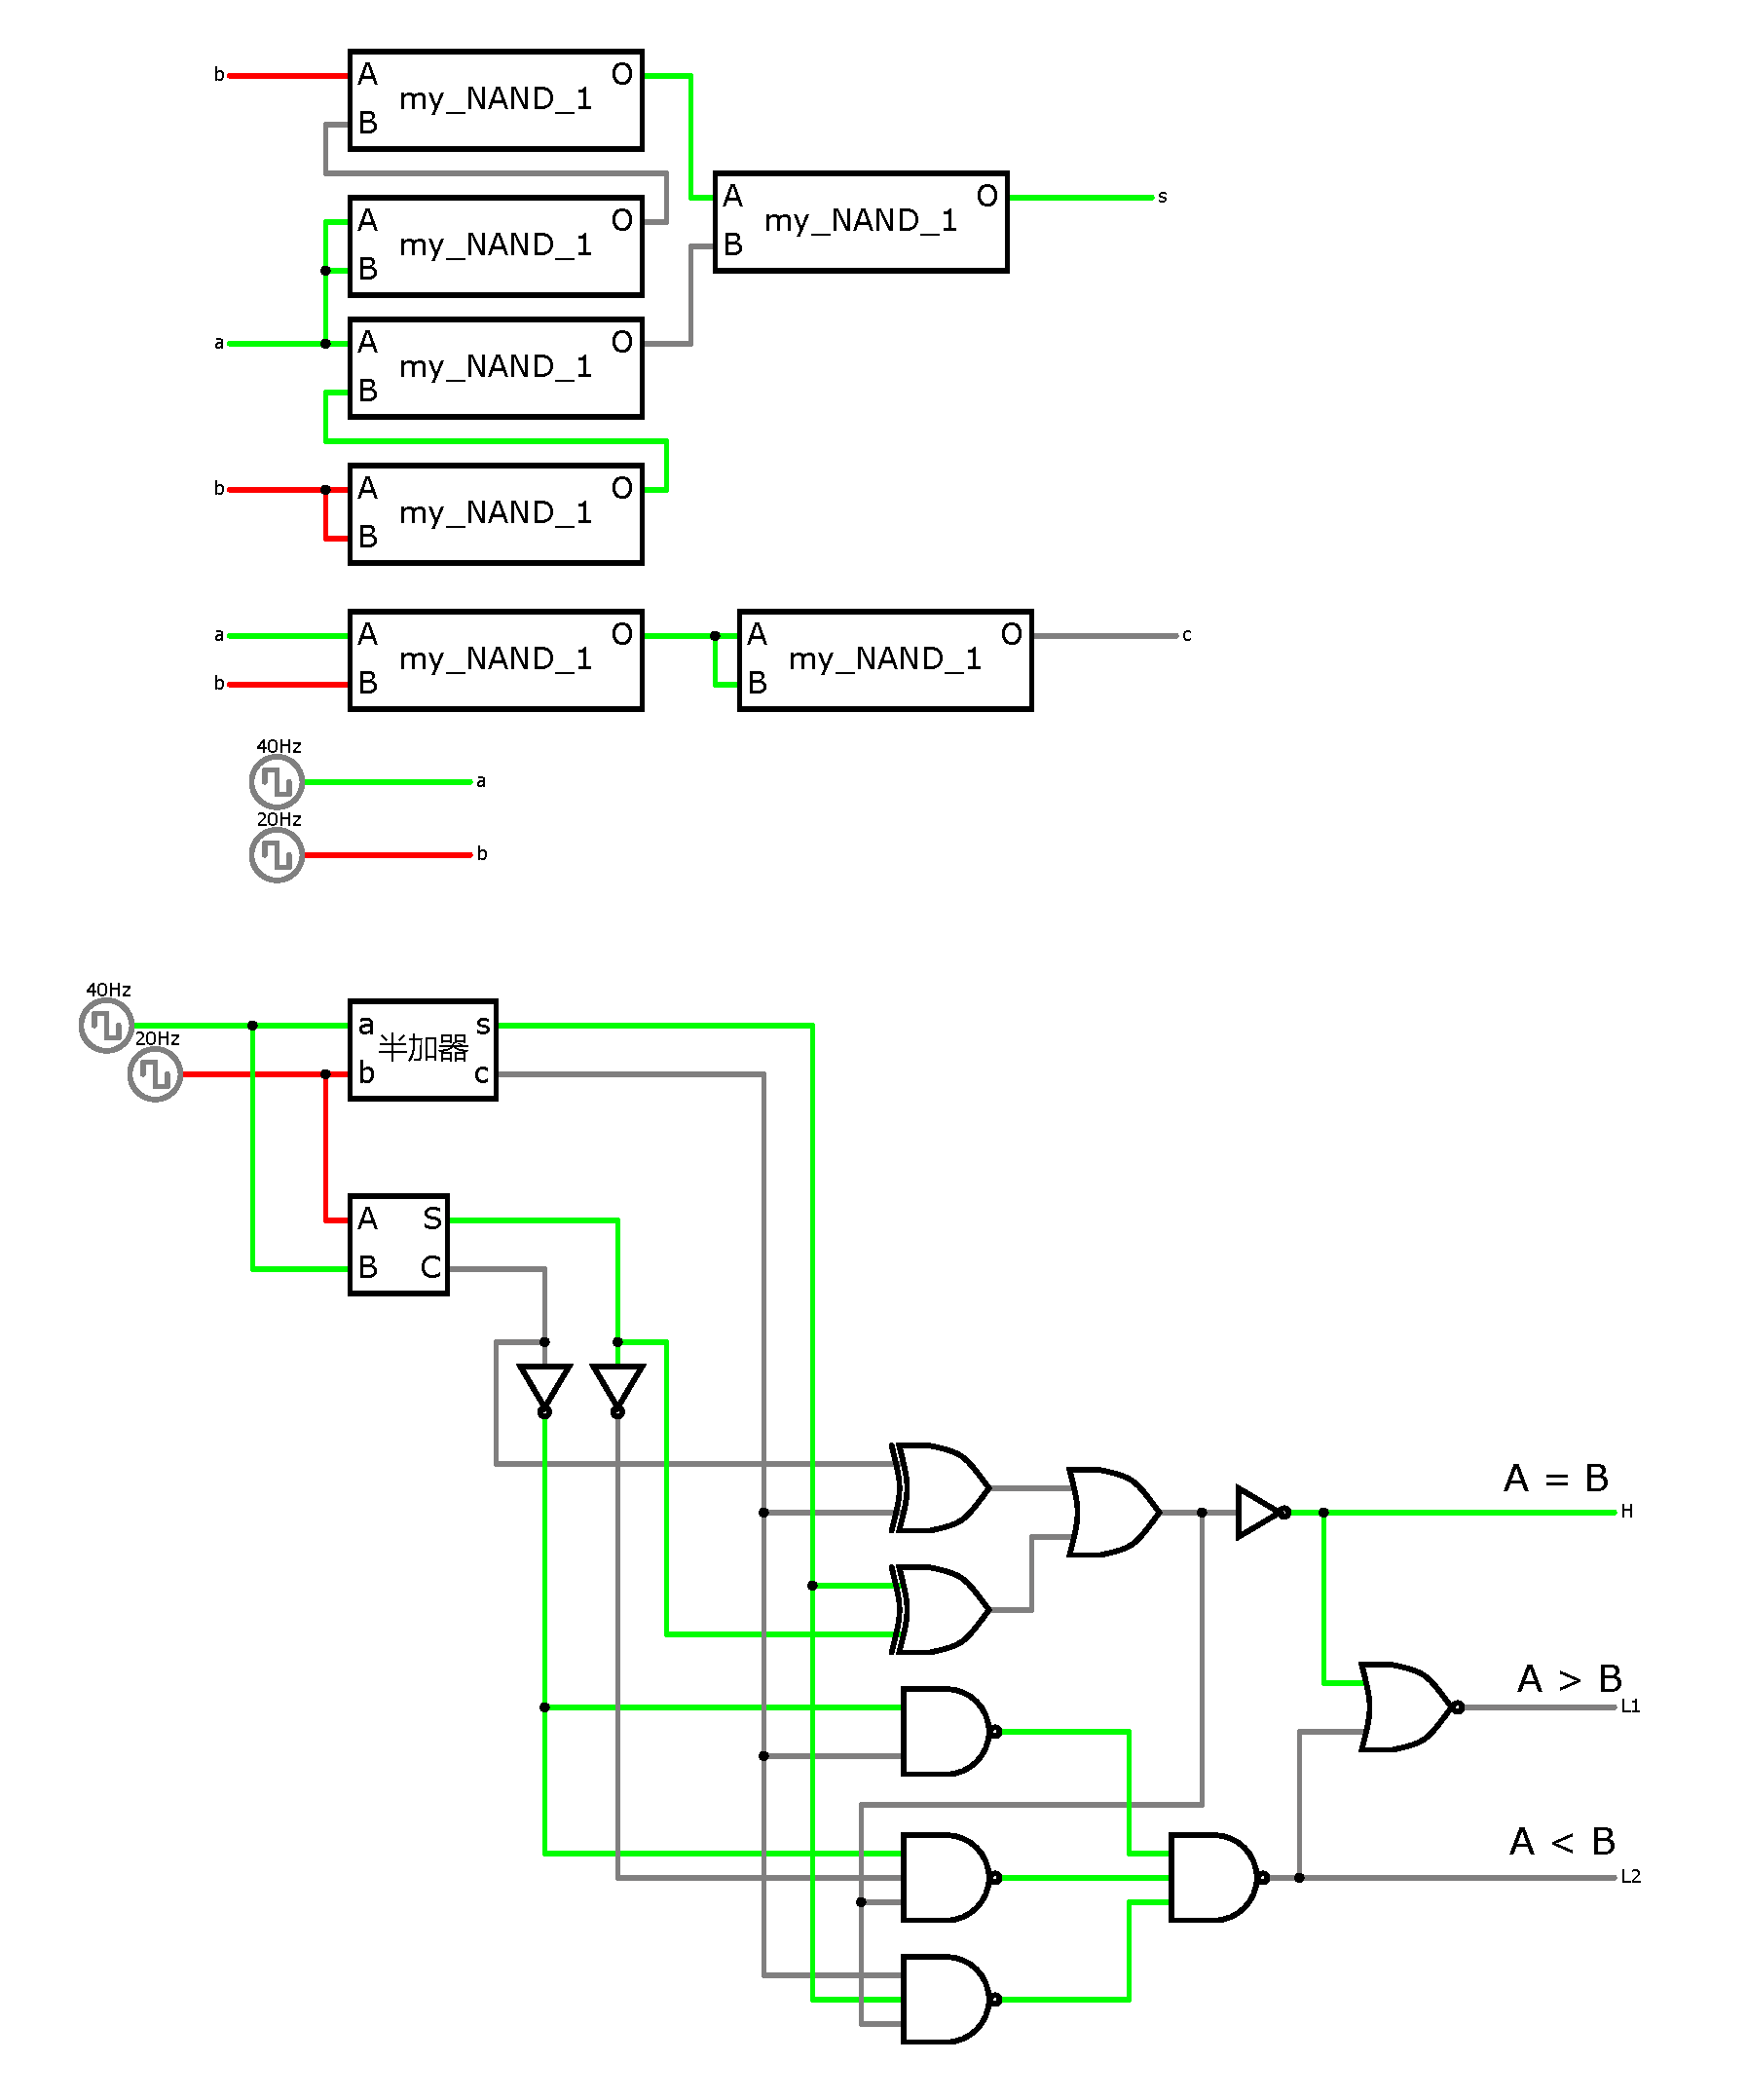
\includegraphics[width=0.7\textwidth]{半加器测试.pdf}
%     \caption{半加器验证与逻辑构建}
% \end{figure}

\begin{figure}[htbp]
    \centering
    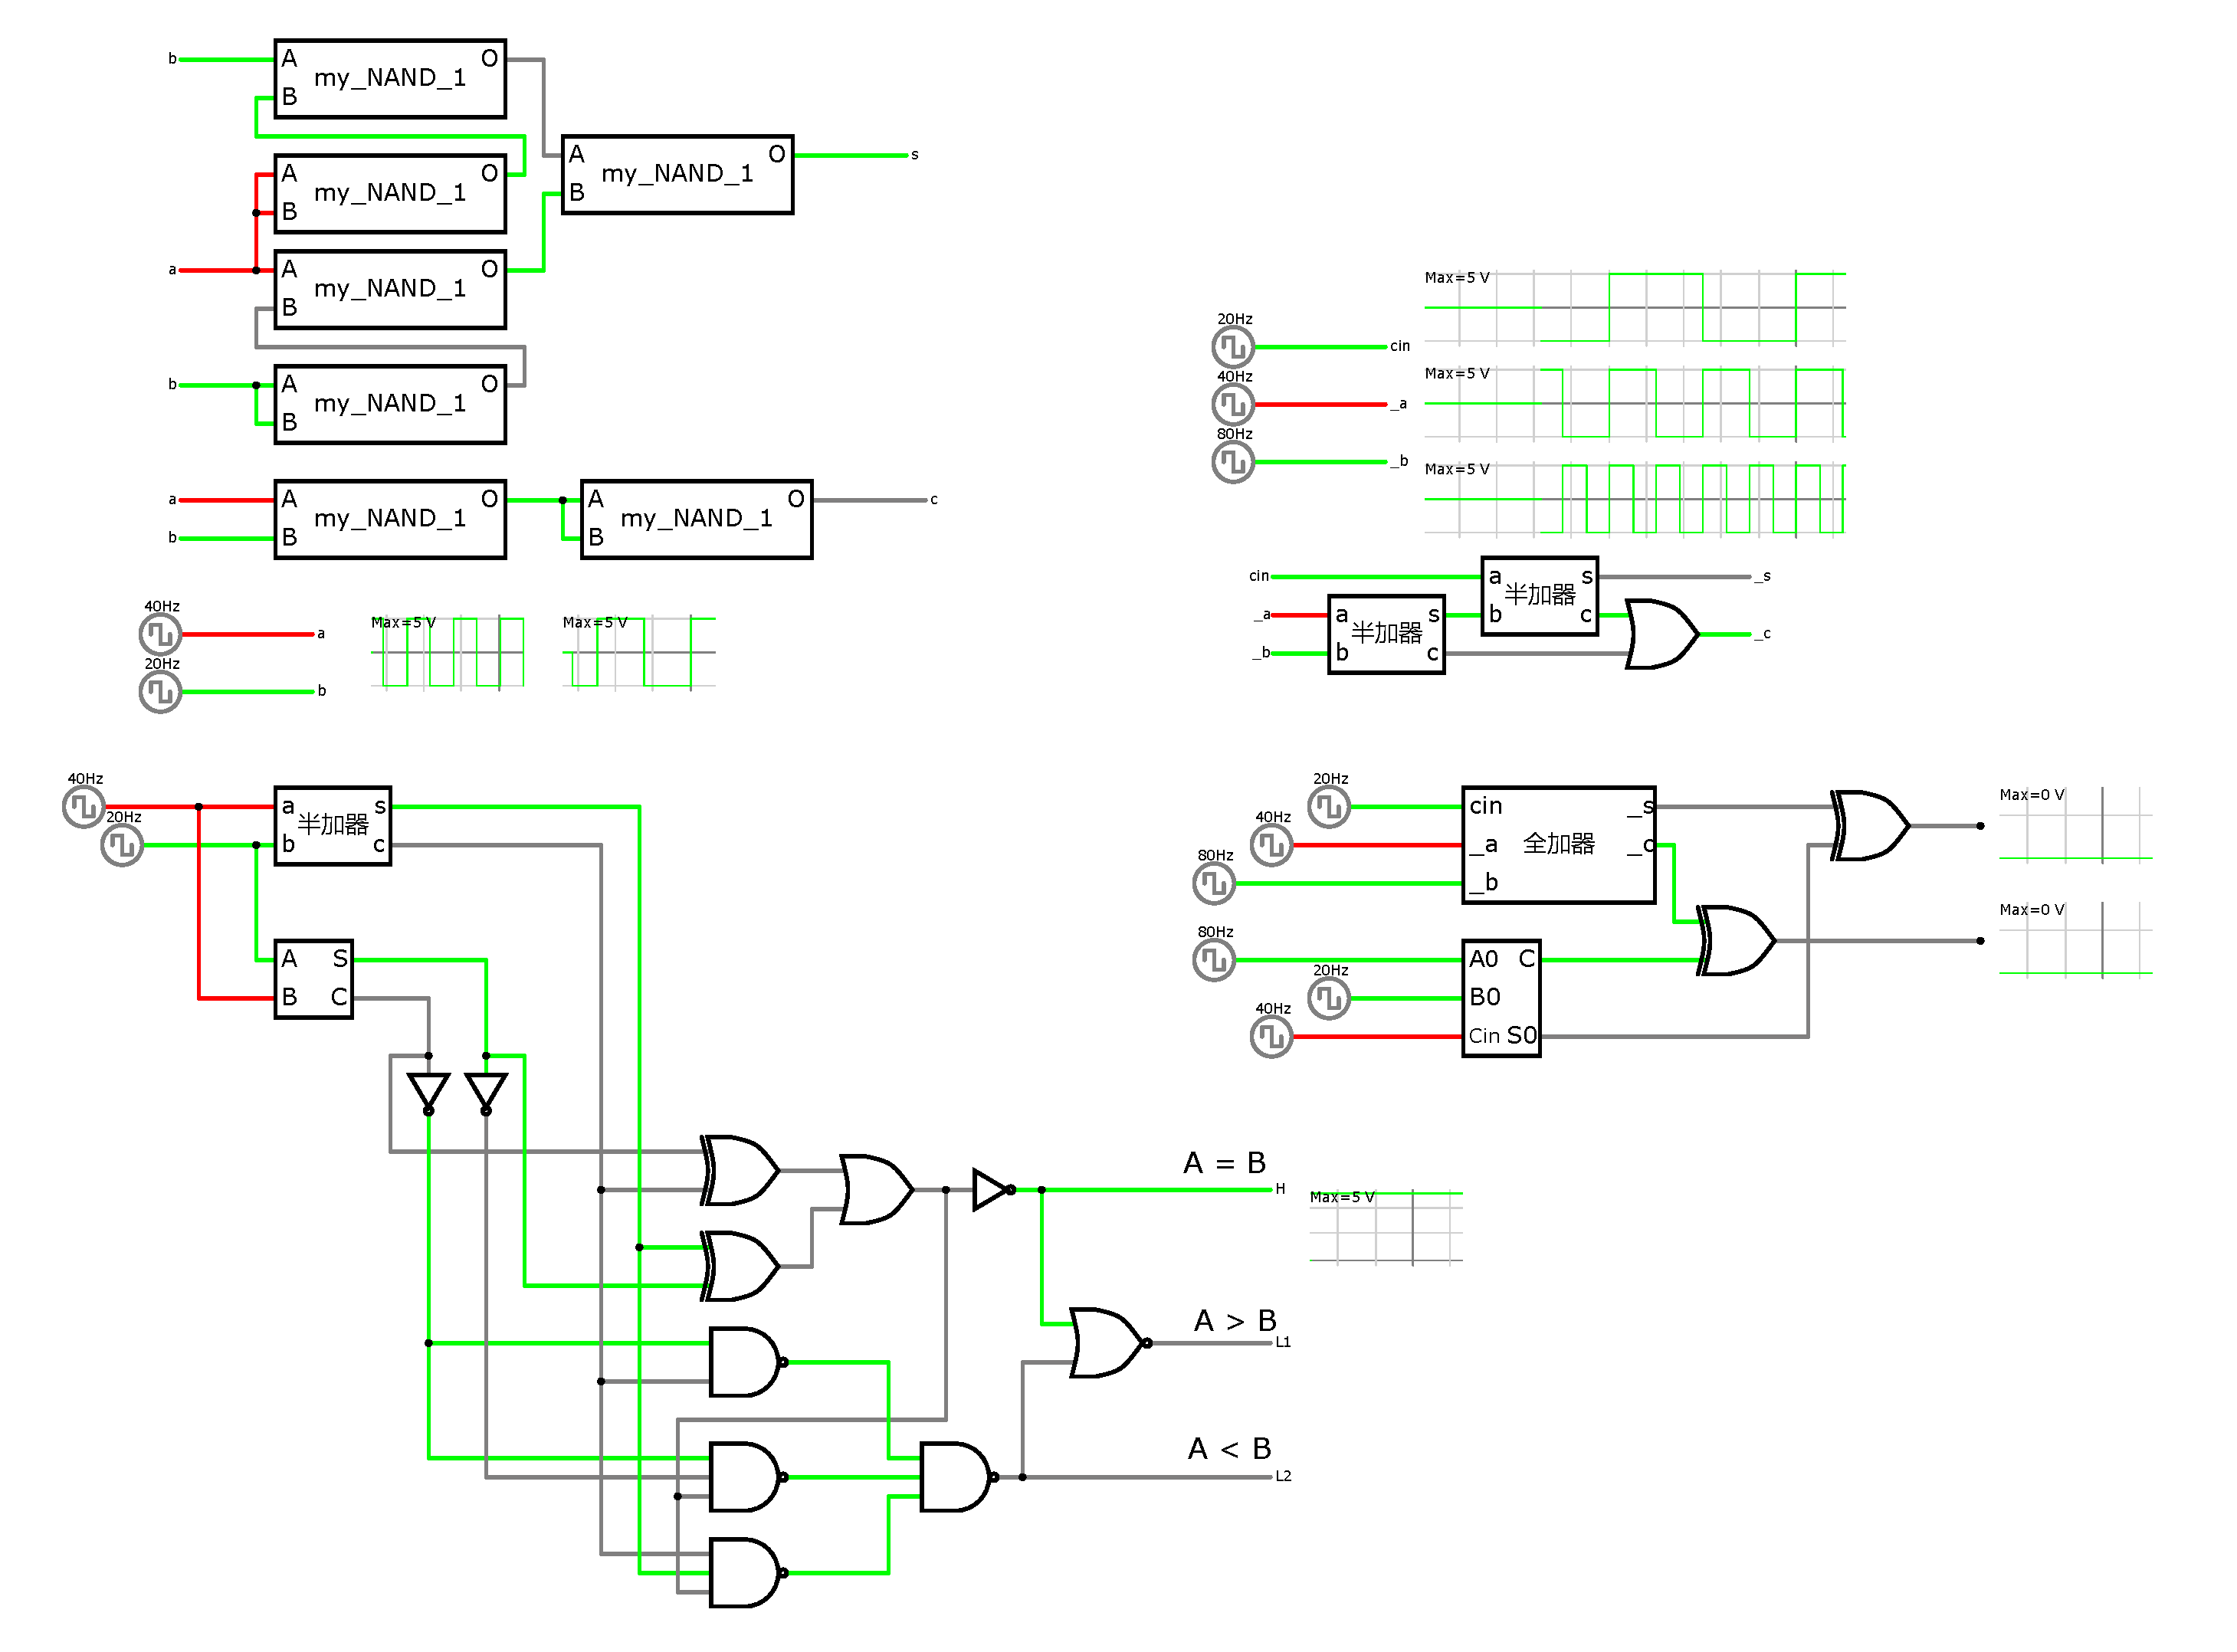
\includegraphics[width=1\textwidth]{半加器与全加器.pdf}
    \caption{半加器与全加器构建}
\end{figure}

\begin{align*}
    \left(\left(\left(\left(\left(\left(\left(\left(1\right)\right)\right)\right)\right)\right)\right)\right)
\end{align*}

\end{document}